\subsection{Fit}\label{fit}

The fit reported here is a population prediction, computed by integrating the estimated model over the opportunity distribution and the taste shocks. It is not a sampled-menu choice probability and it is not an in-sample fitted value. We report it band-referenced: each group's weighted extensive-margin accuracy is compared not to a 100 per cent target -- a correctly specified stochastic-choice model does not attain one -- but to the 95 per cent band that model itself would produce by chance, from 500 outcome vectors simulated at the fitted estimates.

\begin{figure}[H]
\centering
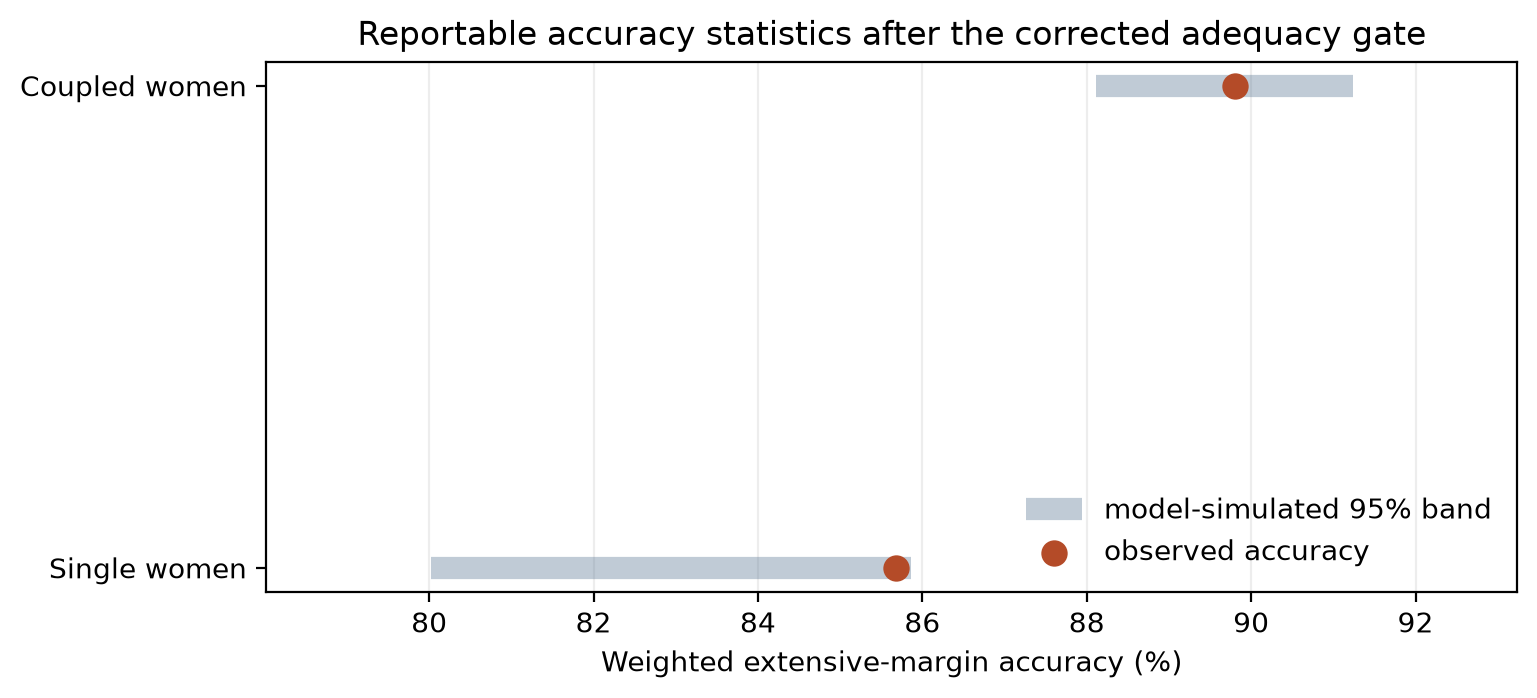
\includegraphics[width=0.95\linewidth,height=\textheight,keepaspectratio,alt={Corrected weighted extensive accuracy. Only single women and coupled women clear the preregistered numerical-adequacy gate. The statistics for single men and coupled men are quadrature-limited and withheld. Source: POSFIT v3b.}]{figures/v7/fitext_band_v3b.png}
\caption{\textbf{Corrected weighted extensive accuracy.} Only single women and coupled women clear the preregistered numerical-adequacy gate. The statistics for single men and coupled men are quadrature-limited and withheld. Source: POSFIT v3b.}
\end{figure}

\begin{figure}[H]
\centering
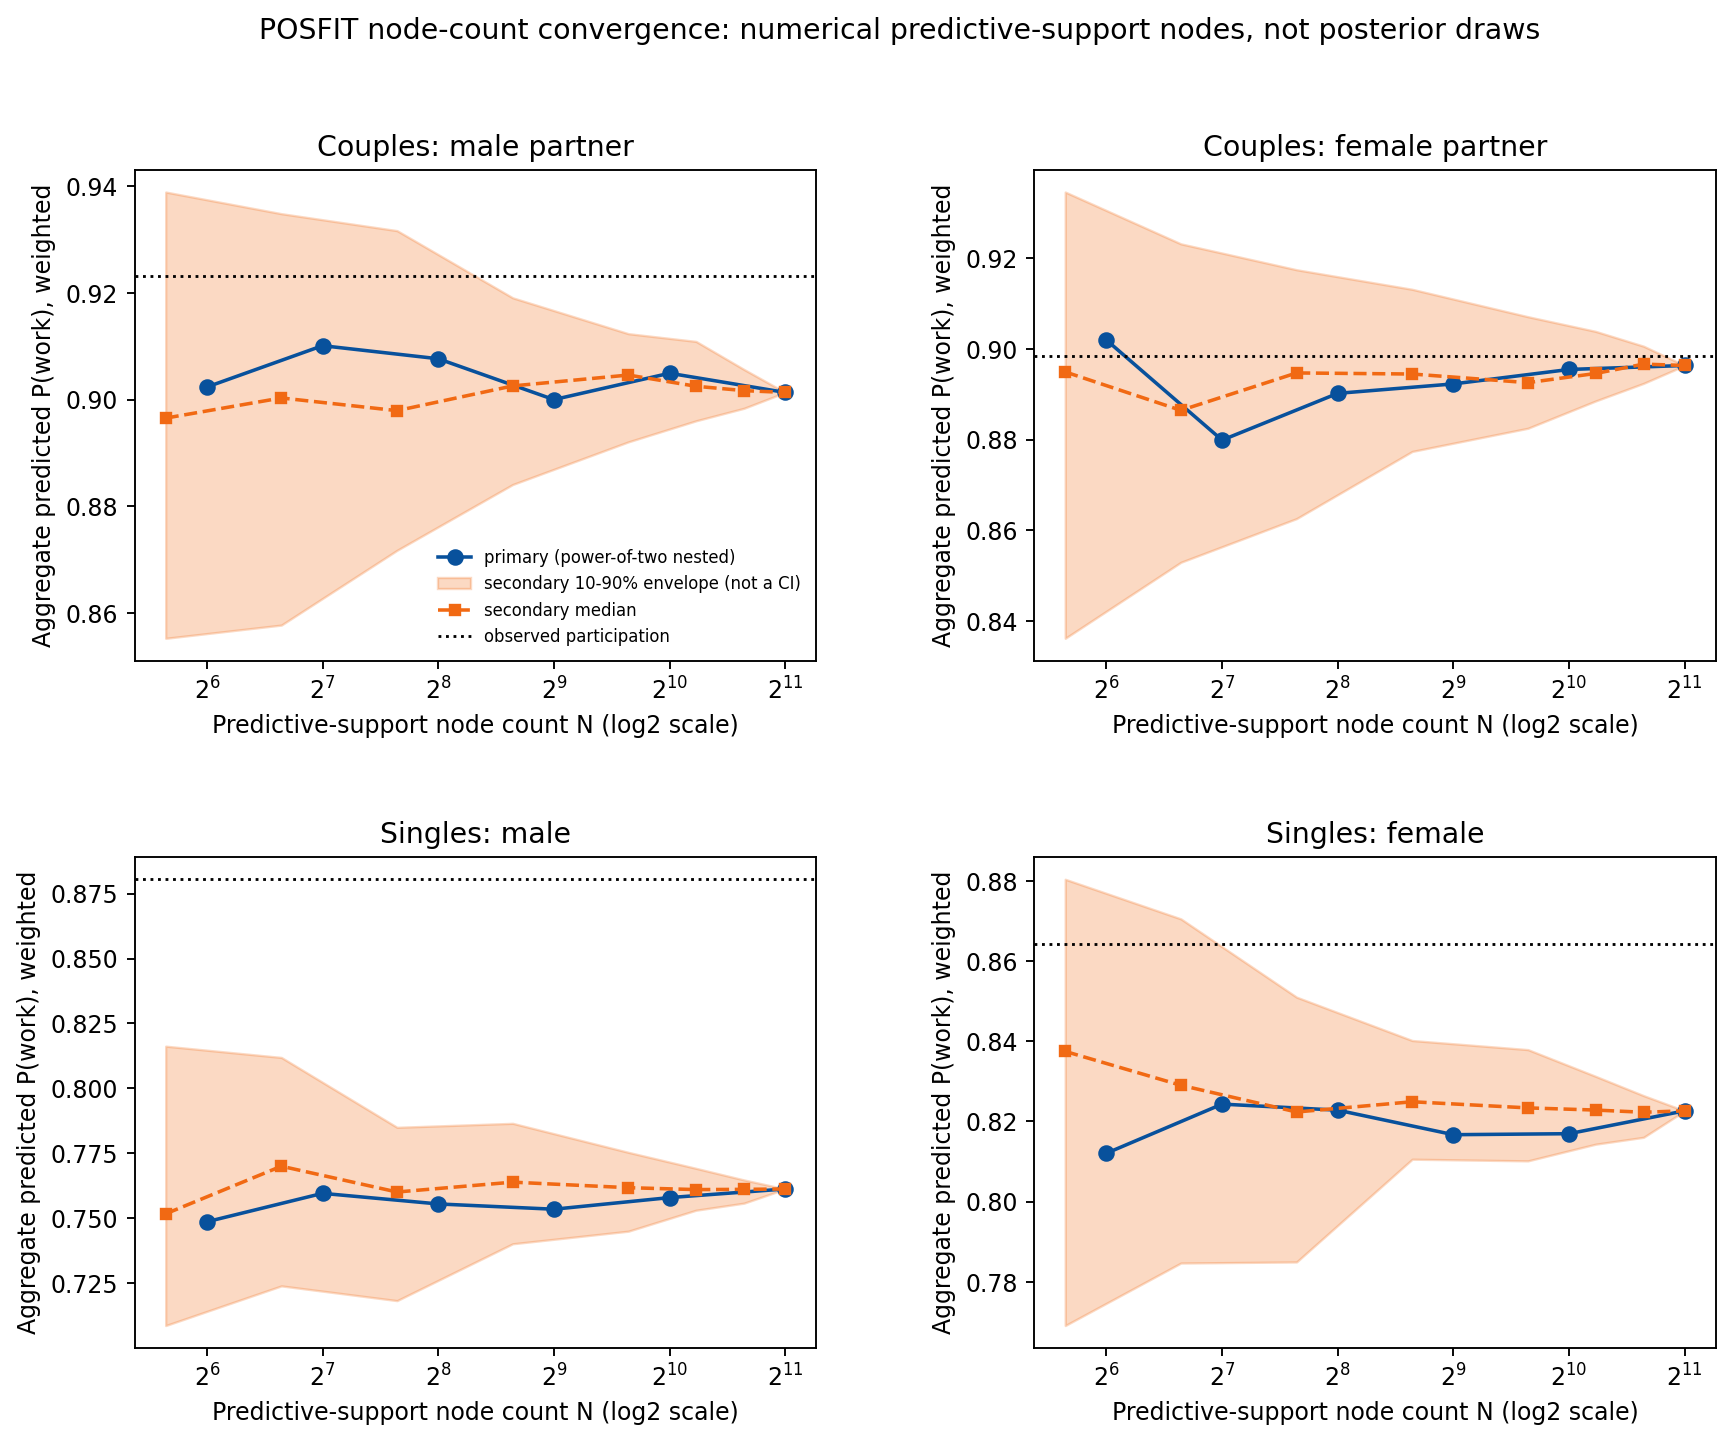
\includegraphics[width=0.95\linewidth,height=\textheight,keepaspectratio,alt={Corrected predictive/integration-node convergence. Weighted predicted participation over fixed-seed node subsets; the shaded area is the numerical 10--90\% envelope and observed participation is the horizontal reference. Source: POSFIT node convergence v3b.}]{figures/v7/node_convergence_v3b.png}
\caption{\textbf{Corrected predictive/integration-node convergence.} Weighted predicted participation over fixed-seed node subsets; the shaded area is the numerical 10--90\% envelope and observed participation is the horizontal reference. Source: POSFIT node convergence v3b.}
\end{figure}

The full reader surface -- all four extensive matrices and four joint hours-state matrices, the four worker-conditional intensive matrices with per-bin statistics, raw counts beside survey-weighted companions, observed-state probability, Brier and log scores, calibration, and the model-simulated benchmark -- is retained in the canonical notebook and results gallery. This report keeps the presentation concise and does not add a group-level fit claim.

Population participation and occupation margins remain close in aggregate, while the corrected hours comparison is uneven. The corrected individual-level diagnostics are adjudicated group by group below; no cross-group excess-predictability headline is maintained.

The corrected POSFIT-v3b numerical-adequacy gate is applied mechanically at the preregistered 0.25 threshold. Single women (85.7\%, simulated 95\% band {[}80.0\%, 85.9\%{]}, ratio 0.096) and coupled women (89.8\%, {[}88.1\%, 91.2\%{]}, ratio 0.049) clear it and are reportable. Single men (ratio 0.361) and coupled men (ratio 0.353) are quadrature-limited, so their extensive accuracy is withheld. In particular, coupled men crossed the threshold after the corrected S11 evaluation and the earlier reportable classification is not preserved.

\subsubsection{The full margin-by-margin comparison}\label{the-full-margin-by-margin-comparison}

\begin{figure}[H]
\centering
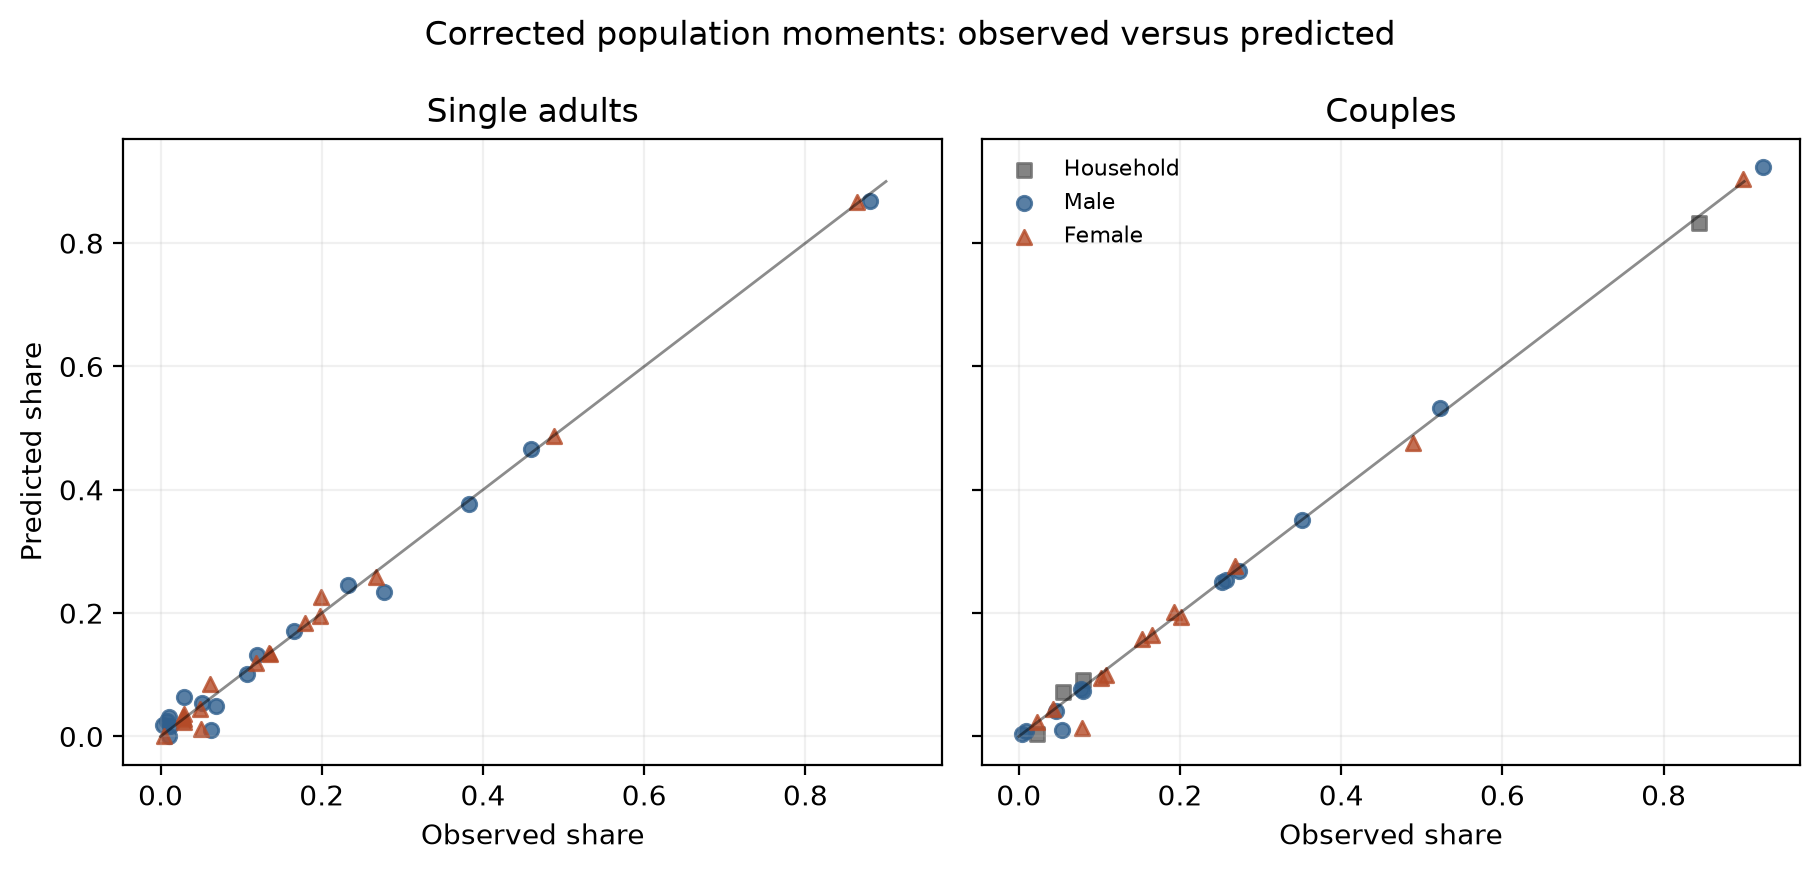
\includegraphics[width=0.95\linewidth,height=\textheight,keepaspectratio,alt={Corrected population fit. Observed against fully re-evaluated S11 model shares using S11/S10 structural-band indicators. The observed 37-hour mass-point cell is a descriptive residual category outside structural FT.}]{figures/v7/fit_by_margin_v7.png}
\caption{\textbf{Corrected population fit.} Observed against fully re-evaluated S11 model shares using S11/S10 structural-band indicators. The observed 37-hour mass-point cell is a descriptive residual category outside structural FT.}
\end{figure}

\Needspace*{12\baselineskip}\small\setlength{\tabcolsep}{3pt}\begin{longtable}[]{@{}
  >{\raggedright\arraybackslash}p{(\linewidth - 10\tabcolsep) * \real{0.1667}}
  >{\raggedright\arraybackslash}p{(\linewidth - 10\tabcolsep) * \real{0.1667}}
  >{\raggedright\arraybackslash}p{(\linewidth - 10\tabcolsep) * \real{0.1667}}
  >{\raggedright\arraybackslash}p{(\linewidth - 10\tabcolsep) * \real{0.1667}}
  >{\raggedright\arraybackslash}p{(\linewidth - 10\tabcolsep) * \real{0.1667}}
  >{\raggedright\arraybackslash}p{(\linewidth - 10\tabcolsep) * \real{0.1667}}@{}}
\caption{Corrected observed against model population moments, singles. Structural PT1, PT2 and FT rows use the S11/S10 definitions; the other hours rows are mutually exclusive descriptive residual categories, including the observed 37-hour mass-point cell. Predictions were fully re-evaluated after rebuilding the structural indicators; no row is a relabelling of the superseded evaluation.}\tabularnewline
\toprule\noalign{}
\begin{minipage}[b]{\linewidth}\raggedright
Unit
\end{minipage} & \begin{minipage}[b]{\linewidth}\raggedright
Moment
\end{minipage} & \begin{minipage}[b]{\linewidth}\raggedright
Observed
\end{minipage} & \begin{minipage}[b]{\linewidth}\raggedright
Model
\end{minipage} & \begin{minipage}[b]{\linewidth}\raggedright
Absolute deviation
\end{minipage} & \begin{minipage}[b]{\linewidth}\raggedright
Denominator
\end{minipage} \\
\midrule\noalign{}
\endfirsthead
\toprule\noalign{}
\begin{minipage}[b]{\linewidth}\raggedright
Unit
\end{minipage} & \begin{minipage}[b]{\linewidth}\raggedright
Moment
\end{minipage} & \begin{minipage}[b]{\linewidth}\raggedright
Observed
\end{minipage} & \begin{minipage}[b]{\linewidth}\raggedright
Model
\end{minipage} & \begin{minipage}[b]{\linewidth}\raggedright
Absolute deviation
\end{minipage} & \begin{minipage}[b]{\linewidth}\raggedright
Denominator
\end{minipage} \\
\midrule\noalign{}
\endhead
\bottomrule\noalign{}
\endlastfoot
Man & Employment & 0.8805 & 0.8675 & 0.0130 & households \\
Man & Hours: non-employment & 0.1195 & 0.1325 & 0.0130 & households \\
Man & Hours: {[}5, 10) & 0.0109 & 0.0000 & 0.0109 & households \\
Man & Hours: {[}10, 18.5) & 0.0080 & 0.0246 & 0.0166 & households \\
Man & Structural PT1: {[}18.5, 21.5) & 0.0113 & 0.0167 & 0.0054 & households \\
Man & Hours: {[}21.5, 29.5) & 0.0286 & 0.0646 & 0.0360 & households \\
Man & Structural PT2: {[}29.5, 30.5) & 0.0032 & 0.0187 & 0.0155 & households \\
Man & Hours: {[}30.5, 33.5) & 0.0107 & 0.0315 & 0.0208 & households \\
Man & Hours: {[}33.5, 36.5) & 0.2329 & 0.2457 & 0.0128 & households \\
Man & Observed 37-hour mass point: {[}36.5, 37.5) & 0.0624 & 0.0105 & 0.0519 & households \\
Man & Structural FT: {[}37.5, 40.5{]} & 0.2776 & 0.2347 & 0.0429 & households \\
Man & Hours: (40.5, 44.5) & 0.0691 & 0.0488 & 0.0203 & households \\
Man & Hours: {[}44.5, 70{]} & 0.1658 & 0.1717 & 0.0059 & households \\
Man & Occupation group 1 & 0.3823 & 0.3774 & 0.0049 & workers \\
Man & Occupation group 2 & 0.1069 & 0.1014 & 0.0054 & workers \\
Man & Occupation group 3 & 0.0516 & 0.0545 & 0.0029 & workers \\
Man & Occupation group 4 & 0.4593 & 0.4667 & 0.0074 & workers \\
Man & Mean log wage & 2.6876 & 2.6309 & 0.0567 & workers \\
Woman & Employment & 0.8642 & 0.8665 & 0.0024 & households \\
Woman & Hours: non-employment & 0.1358 & 0.1335 & 0.0024 & households \\
Woman & Hours: {[}5, 10) & 0.0042 & 0.0000 & 0.0042 & households \\
Woman & Hours: {[}10, 18.5) & 0.0278 & 0.0317 & 0.0038 & households \\
Woman & Structural PT1: {[}18.5, 21.5) & 0.0290 & 0.0283 & 0.0007 & households \\
Woman & Hours: {[}21.5, 29.5) & 0.0612 & 0.0856 & 0.0245 & households \\
Woman & Structural PT2: {[}29.5, 30.5) & 0.0288 & 0.0236 & 0.0052 & households \\
Woman & Hours: {[}30.5, 33.5) & 0.0290 & 0.0367 & 0.0077 & households \\
Woman & Hours: {[}33.5, 36.5) & 0.2672 & 0.2581 & 0.0091 & households \\
Woman & Observed 37-hour mass point: {[}36.5, 37.5) & 0.0503 & 0.0123 & 0.0381 & households \\
Woman & Structural FT: {[}37.5, 40.5{]} & 0.1990 & 0.2264 & 0.0274 & households \\
Woman & Hours: (40.5, 44.5) & 0.0492 & 0.0446 & 0.0045 & households \\
Woman & Hours: {[}44.5, 70{]} & 0.1185 & 0.1192 & 0.0007 & households \\
Woman & Occupation group 1 & 0.1795 & 0.1832 & 0.0036 & workers \\
Woman & Occupation group 2 & 0.1976 & 0.1946 & 0.0031 & workers \\
Woman & Occupation group 3 & 0.1349 & 0.1348 & 0.0002 & workers \\
Woman & Occupation group 4 & 0.4879 & 0.4875 & 0.0004 & workers \\
Woman & Mean log wage & 2.5968 & 2.6207 & 0.0238 & workers \\
\end{longtable}

\Needspace*{12\baselineskip}\small\setlength{\tabcolsep}{3pt}\begin{longtable}[]{@{}
  >{\raggedright\arraybackslash}p{(\linewidth - 10\tabcolsep) * \real{0.1667}}
  >{\raggedright\arraybackslash}p{(\linewidth - 10\tabcolsep) * \real{0.1667}}
  >{\raggedright\arraybackslash}p{(\linewidth - 10\tabcolsep) * \real{0.1667}}
  >{\raggedright\arraybackslash}p{(\linewidth - 10\tabcolsep) * \real{0.1667}}
  >{\raggedright\arraybackslash}p{(\linewidth - 10\tabcolsep) * \real{0.1667}}
  >{\raggedright\arraybackslash}p{(\linewidth - 10\tabcolsep) * \real{0.1667}}@{}}
\caption{Corrected observed against model population moments, couples. Structural PT1, PT2 and FT rows use the S11/S10 definitions; the other hours rows are mutually exclusive descriptive residual categories, including the observed 37-hour mass-point cell. Predictions were fully re-evaluated after rebuilding the structural indicators; no row is a relabelling of the superseded evaluation.}\tabularnewline
\toprule\noalign{}
\begin{minipage}[b]{\linewidth}\raggedright
Unit
\end{minipage} & \begin{minipage}[b]{\linewidth}\raggedright
Moment
\end{minipage} & \begin{minipage}[b]{\linewidth}\raggedright
Observed
\end{minipage} & \begin{minipage}[b]{\linewidth}\raggedright
Model
\end{minipage} & \begin{minipage}[b]{\linewidth}\raggedright
Absolute deviation
\end{minipage} & \begin{minipage}[b]{\linewidth}\raggedright
Denominator
\end{minipage} \\
\midrule\noalign{}
\endfirsthead
\toprule\noalign{}
\begin{minipage}[b]{\linewidth}\raggedright
Unit
\end{minipage} & \begin{minipage}[b]{\linewidth}\raggedright
Moment
\end{minipage} & \begin{minipage}[b]{\linewidth}\raggedright
Observed
\end{minipage} & \begin{minipage}[b]{\linewidth}\raggedright
Model
\end{minipage} & \begin{minipage}[b]{\linewidth}\raggedright
Absolute deviation
\end{minipage} & \begin{minipage}[b]{\linewidth}\raggedright
Denominator
\end{minipage} \\
\midrule\noalign{}
\endhead
\bottomrule\noalign{}
\endlastfoot
Household & Joint regime neither works & 0.0222 & 0.0043 & 0.0178 & households \\
Household & Joint regime man only & 0.0794 & 0.0909 & 0.0115 & households \\
Household & Joint regime woman only & 0.0547 & 0.0723 & 0.0176 & households \\
Household & Joint regime both work & 0.8437 & 0.8324 & 0.0113 & households \\
Man & Employment & 0.9231 & 0.9234 & 0.0002 & households \\
Man & Hours: non-employment & 0.0769 & 0.0766 & 0.0002 & households \\
Man & Structural PT1: {[}18.5, 21.5) & 0.0037 & 0.0041 & 0.0004 & households \\
Man & Structural PT2: {[}29.5, 30.5) & 0.0093 & 0.0094 & 0.0002 & households \\
Man & Hours: {[}33.5, 36.5) & 0.2515 & 0.2507 & 0.0008 & households \\
Man & Observed 37-hour mass point: {[}36.5, 37.5) & 0.0539 & 0.0098 & 0.0441 & households \\
Man & Structural FT: {[}37.5, 40.5{]} & 0.2736 & 0.2682 & 0.0054 & households \\
Man & Hours: {[}44.5, 70{]} & 0.2576 & 0.2531 & 0.0044 & households \\
Man & Occupation group 1 & 0.3519 & 0.3516 & 0.0003 & workers \\
Man & Occupation group 2 & 0.0797 & 0.0741 & 0.0056 & workers \\
Man & Occupation group 3 & 0.0464 & 0.0412 & 0.0052 & workers \\
Man & Occupation group 4 & 0.5220 & 0.5331 & 0.0111 & workers \\
Man & Mean log wage & 2.7687 & 2.7054 & 0.0633 & workers \\
Woman & Employment & 0.8984 & 0.9047 & 0.0063 & households \\
Woman & Hours: non-employment & 0.1016 & 0.0953 & 0.0063 & households \\
Woman & Structural PT1: {[}18.5, 21.5) & 0.0229 & 0.0230 & 0.0001 & households \\
Woman & Structural PT2: {[}29.5, 30.5) & 0.0419 & 0.0439 & 0.0020 & households \\
Woman & Hours: {[}33.5, 36.5) & 0.2687 & 0.2767 & 0.0080 & households \\
Woman & Observed 37-hour mass point: {[}36.5, 37.5) & 0.0785 & 0.0134 & 0.0651 & households \\
Woman & Structural FT: {[}37.5, 40.5{]} & 0.2008 & 0.1938 & 0.0070 & households \\
Woman & Hours: {[}44.5, 70{]} & 0.1079 & 0.1002 & 0.0077 & households \\
Woman & Occupation group 1 & 0.1653 & 0.1648 & 0.0005 & workers \\
Woman & Occupation group 2 & 0.1922 & 0.2017 & 0.0095 & workers \\
Woman & Occupation group 3 & 0.1533 & 0.1583 & 0.0050 & workers \\
Woman & Occupation group 4 & 0.4892 & 0.4752 & 0.0140 & workers \\
Woman & Mean log wage & 2.6072 & 2.6319 & 0.0247 & workers \\
\end{longtable}

The corrected mean absolute deviation over all population moments is 0.0140 across 36 single-adult moments and 0.0119 across 30 couple moments. This correction is not an across-the-board fit improvement: singles MAE rises slightly, while couples MAE falls. The remaining common mismatch is underprediction of the observed 37-hour mass point, by 3.8--6.5 percentage points across the four groups. That mass point lies outside the S11 structural full-time band \([37.5,40.5]\); it is not described as underprediction of that structural band. The sub-ten-hour cell remains a finite-integration-panel coverage limitation, and the long-hours reporting bin closes at 70 inclusive.

\Needspace*{12\baselineskip}\small\setlength{\tabcolsep}{3pt}\begin{longtable}[]{@{}
  >{\raggedright\arraybackslash}p{(\linewidth - 8\tabcolsep) * \real{0.2000}}
  >{\raggedright\arraybackslash}p{(\linewidth - 8\tabcolsep) * \real{0.2000}}
  >{\raggedright\arraybackslash}p{(\linewidth - 8\tabcolsep) * \real{0.2000}}
  >{\raggedright\arraybackslash}p{(\linewidth - 8\tabcolsep) * \real{0.2000}}
  >{\raggedright\arraybackslash}p{(\linewidth - 8\tabcolsep) * \real{0.2000}}@{}}
\caption{The estimated singles model against two re-estimated common-opportunity benchmarks. Estimates and maximized criteria are unchanged; criterion-B population moments are corrected to the S11/S10 structural-band definitions. The RUM-A estimation-input band defect and its cancellation in the conditional likelihood are disclosed in the limitations.}\tabularnewline
\toprule\noalign{}
\begin{minipage}[b]{\linewidth}\raggedright
Specification
\end{minipage} & \begin{minipage}[b]{\linewidth}\raggedright
Free coordinates
\end{minipage} & \begin{minipage}[b]{\linewidth}\raggedright
Criterion
\end{minipage} & \begin{minipage}[b]{\linewidth}\raggedright
Difference
\end{minipage} & \begin{minipage}[b]{\linewidth}\raggedright
Population fit
\end{minipage} \\
\midrule\noalign{}
\endfirsthead
\toprule\noalign{}
\begin{minipage}[b]{\linewidth}\raggedright
Specification
\end{minipage} & \begin{minipage}[b]{\linewidth}\raggedright
Free coordinates
\end{minipage} & \begin{minipage}[b]{\linewidth}\raggedright
Criterion
\end{minipage} & \begin{minipage}[b]{\linewidth}\raggedright
Difference
\end{minipage} & \begin{minipage}[b]{\linewidth}\raggedright
Population fit
\end{minipage} \\
\midrule\noalign{}
\endhead
\bottomrule\noalign{}
\endlastfoot
Latent jobs with household-specific opportunities & 41 & 6253.463 & -- & 0.0140 \\
Benchmark A: common opportunity distribution, preferences re-estimated & 10 & 6403.974 & +150.51 & 0.0273 \\
Benchmark B: common opportunity shape, employment and hours moved into utility & 16 & 6395.108 & +141.64 & 0.0264 \\
\end{longtable}

The two re-estimated common-opportunity benchmarks are worse by 141.64 and by a larger margin, on the same households, the same sampled alternatives and the same criterion. The comparison is a nested one in the sense that the benchmarks restrict the opportunity block and re-estimate everything else, but we do not convert it into a formal test, because the sampled-alternative criterion is not the likelihood of the observed data and the conditions for a likelihood-ratio distribution are not established here. What the table does support is that the deterioration is concentrated where the opportunity block does its work: the population fit worsens from 0.0140 to 0.0273 and 0.0264, and the occupation margins deteriorate by an order of magnitude, from about half a percentage point to eleven. A better criterion does not by itself establish that a mechanism has been identified.

